\section{Desarrollo}
\label{sec_3}

\subsection{Plantilla de Requerimientos}
\label{sec_3.0}
La plantilla de la Cátedra \cite{guia} establece los siguientes requerimientos:
\begin{itemize}
    \item \underline{Banda de paso:} $f_{p1} = 800 \, [Hz]$ a $f_{p2} = 1250 \, [Hz]$, con atenuación máxima $A_p = 0.25 \, [dB]$.
    \item \underline{Bandas de rechazo:} $f < f_{s1} = 200 \, [Hz]$ y $f > f_{s2} = 5000 \, [Hz]$, con atenuación mínima $A_s = 30 \, [dB]$.
\end{itemize}

Se observa que $f_{s1} \, f_{s2} = f_{p1} \, f_{p2} = 10^6 \, [Hz^2]$, es decir, la plantilla es geométricamente simétrica respecto de la frecuencia central $f_0 = \sqrt{f_{p1} f_{p2}} = 1000 \, [Hz]$. Todos los cálculos numéricos se realizaron en Python con la biblioteca \textit{SciPy}, cuyas funciones \texttt{cheb1ord} y \texttt{cheby1} son equivalentes a las de Matlab propuestas en el anexo de la guía; los scripts se encuentran en la carpeta \texttt{TP4/scripts} del repositorio.

\subsection{Aproximación de Chebyshev}
\label{sec_3.1}
A partir de la \autoref{eq:eps}, el parámetro de rizado es:
\begin{equation}
    \varepsilon = \sqrt{10^{0.25/10} - 1} = 0.2434
\end{equation}

El ancho de banda es $B = 2\pi \, (1250 - 800) = 2827.43 \, [rad/s]$ y la frecuencia central $\omega_0 = 2\pi \cdot 1000 = 6283.19 \, [rad/s]$. Por la simetría geométrica de la plantilla, ambos bordes de rechazo conducen a la misma frecuencia normalizada (\autoref{eq:omegas}):
\begin{equation}
    \Omega_s = \frac{5000^2 - 1000^2}{5000 \cdot 450} = \frac{1000^2 - 200^2}{200 \cdot 450} = 10.67
\end{equation}

Reemplazando en la \autoref{eq:orden}:
\begin{equation}
    n \geq \frac{\mathrm{arccosh}\sqrt{\dfrac{10^{3} - 1}{10^{0.025} - 1}}}{\mathrm{arccosh} \, 10.67} = \frac{5.560}{3.059} = 1.82 \quad \Rightarrow \quad n = 2
\end{equation}

El prototipo pasabajos normalizado de Chebyshev de orden $2$ con $A_p = 0.25 \, [dB]$ resulta:
\begin{equation}
    H_{LP}(s) = \frac{2.0541}{s^2 + 1.7967 \, s + 2.1140}
\end{equation}
cuya ganancia en continua es $2.0541/2.1140 = 0.9717$ ($-0.25 \, [dB]$), como corresponde a un filtro de Chebyshev de orden par. Aplicando la transformación de la \autoref{eq:transf} se obtiene el pasabanda de orden $4$:
\begin{equation}
    T(s) = \frac{1.64209 \times 10^{7} \, s^2}{s^4 + 5080.00 \, s^3 + 9.58572 \times 10^{7} \, s^2 + 2.00550 \times 10^{11} \, s + 1.55855 \times 10^{15}}
    \label{eq:T}
\end{equation}

Los polos de la \autoref{eq:T} y sus parámetros se presentan en la \autoref{tab:polos}. Factorizando, la función de transferencia coincide con la indicada en la plantilla de la Cátedra:
\begin{equation}
    T(s) = \frac{5252.26 \, s}{s^2 + 3184.42 \, s + 66320656} \cdot \frac{3126.49 \, s}{s^2 + 1895.58 \, s + 23500096}
\end{equation}

\begin{table}[H]
    \centering
    \caption{Polos de la función de transferencia aproximada.}
    \label{tab:polos}
    \begin{tabular}{|c|c|c|c|c|}
        \hline
        \textbf{Par de polos} & \textbf{Ubicación $[rad/s]$} & $\boldsymbol{f_p \, [Hz]}$ & $\boldsymbol{Q_p}$ & $\boldsymbol{\omega_p / Q_p \, [rad/s]}$ \\
        \hline
        Bajo & $-947.79 \pm j \, 4754.13$  & $771.53$  & $2.557$ & $1895.58$ \\
        Alto & $-1592.21 \pm j \, 7986.59$ & $1296.12$ & $2.557$ & $3184.43$ \\
        \hline
    \end{tabular}
\end{table}

Ambos pares tienen el mismo factor de calidad, consecuencia de la simetría geométrica de la transformación pasabanda. La atenuación en $200 \, [Hz]$ y en $5 \, [kHz]$ es de $34.83 \, [dB]$, de modo que el orden $2$ satisface la plantilla con un margen de $4.83 \, [dB]$ en la banda de rechazo. La respuesta se muestra en la \autoref{fig:aprox}.

\begin{figure}[H]
    \centering
    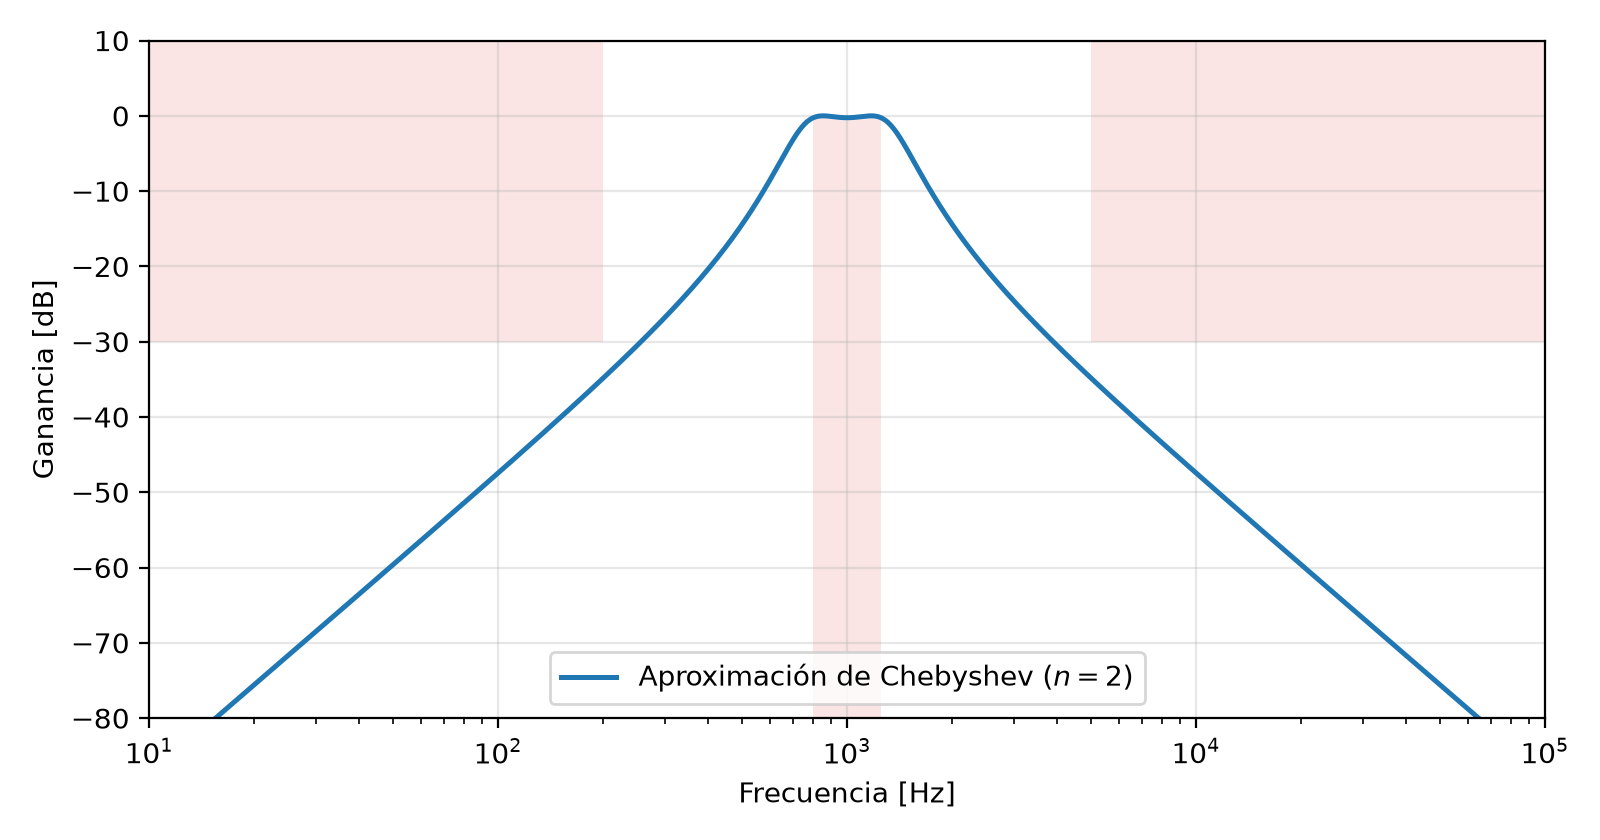
\includegraphics[width=0.85\textwidth]{aproximacion_chebyshev.png}
    \caption{Respuesta en frecuencia de la aproximación de Chebyshev y de cada etapa, junto con la plantilla de requerimientos (zonas sombreadas).}
    \label{fig:aprox}
\end{figure}

\subsection{Síntesis del Circuito}
\label{sec_3.2}

\subsubsection{Descomposición en Bicuadráticas}
Siguiendo la propuesta del anexo de la guía, la función de transferencia se implementa como la cascada de un pasabajos y un pasaaltos de segundo orden. El numerador $K s^2$ admite dos asignaciones de los pares de polos; se elige asignar el par bajo al pasabajos y el par alto al pasaaltos:
\begin{equation}
    T(s) = \underbrace{\frac{\alpha \, \omega_L^2}{s^2 + \dfrac{\omega_L}{Q} s + \omega_L^2}}_{\text{Pasabajos}} \cdot \underbrace{\frac{s^2}{s^2 + \dfrac{\omega_H}{Q} s + \omega_H^2}}_{\text{Pasaaltos}},
    \qquad \alpha = \frac{K}{\omega_L^2} = \frac{1.64209 \times 10^7}{23500096} = 0.6988
    \label{eq:alfa}
\end{equation}

Con esta asignación, dos etapas de ganancia unitaria producirían una ganancia de $1/\alpha = +3.11 \, [dB]$ en la banda de paso, por lo que basta una atenuación de entrada de $\alpha = -3.11 \, [dB]$ para normalizarla. La asignación opuesta exigiría $\alpha = K / \omega_H^2 = 0.2476$ ($-12.1 \, [dB]$), con mayores ganancias internas y menor rango dinámico.

La atenuación $\alpha$ se obtiene reemplazando $R_1$ del pasabajos por un divisor resistivo $R_a$--$R_b$ cuyo equivalente de Thévenin es:
\begin{equation}
    R_1 = R_a \parallel R_b, \qquad \alpha = \frac{R_b}{R_a + R_b} \qquad \Rightarrow \qquad R_a = \frac{R_1}{\alpha}, \qquad R_b = \frac{R_1}{1 - \alpha}
\end{equation}
de forma que no se agregan componentes activos ni se modifican $\omega_p$ y $Q_p$.

\subsubsection{Etapa Pasabajos}
De la \autoref{eq:q_cociente}, para $Q = 2.557$ se requiere $C_1 / C_2 = 4 Q^2 = 26.16$. Se eligen capacitores de la serie E12 $C_1 = 47 \, [nF]$ y $C_2 = 1.8 \, [nF]$ (cociente $26.11$), y con ellos:
\begin{equation}
    R = \frac{1}{\omega_L \sqrt{C_1 C_2}} = \frac{1}{4847.69 \cdot \sqrt{47 \, [nF] \cdot 1.8 \, [nF]}} = 22.43 \, [k\Omega]
\end{equation}

Para minimizar el error al normalizar las resistencias a la serie E96 ($1 \, [\%]$), se realizó una búsqueda sobre los valores normalizados vecinos admitiendo $R_1 \neq R_2$, lo que permite corregir levemente $Q_p$ mediante el cociente $R_1/R_2$ (\autoref{eq:sk_pb}). Se obtuvo $R_2 = 23.2 \, [k\Omega]$, $R_a = 30.9 \, [k\Omega]$ y $R_b = 73.2 \, [k\Omega]$ ($R_1 = 21.73 \, [k\Omega]$, $\alpha = 0.703$).

\subsubsection{Etapa Pasaaltos}
De la \autoref{eq:q_cociente}, $R_4 / R_3 = 4 Q^2 = 26.16$. Con $C_3 = C_4 = 12 \, [nF]$:
\begin{equation}
    \sqrt{R_3 R_4} = \frac{1}{\omega_H \, C} = 10.23 \, [k\Omega] \qquad \Rightarrow \qquad R_3 = 2.00 \, [k\Omega], \quad R_4 = 52.3 \, [k\Omega]
\end{equation}

\subsubsection{Circuito Final}
El circuito completo se muestra en la \autoref{fig:circuito}, y la \autoref{tab:componentes} compara los parámetros obtenidos con los valores normalizados frente a los teóricos. Los amplificadores operacionales son LM324 \cite{lm324} alimentados con $\pm 12 \, [V]$.

\begin{figure}[H]
    \centering
    \begin{circuitikz}[scale=0.62, transform shape]
        \draw (8.8,0) node[op amp, noinv input up, anchor=+] (U1) {$U_1$};
        \draw (0,0) node[left]{$V_{in}$} to[R, l=$R_a$, a=$30.9 \, k\Omega$, o-*] (2.6,0) to[R, l=$R_2$, a=$23.2 \, k\Omega$, -*] (5.4,0) -- (U1.+);
        \draw (2.6,0) to[R, l_={$R_b = 73.2 \, k\Omega$}] (2.6,-2.2) node[ground]{};
        \draw (5.4,0) to[C, l^={$C_2 = 1.8 \, nF$}] (5.4,-2.2) node[ground]{};
        \draw (2.6,0) -- (2.6,2.2) to[C, l=$C_1$, a=$47 \, nF$] ($(U1.out)+(0.6,2.7)$) -- ($(U1.out)+(0.6,0)$);
        \draw (U1.-) -- ++(-0.3,0) |- ($(U1.out)+(0,-1.3)$) -- (U1.out);
        \draw (U1.out) to[short, -*] ($(U1.out)+(0.6,0)$) to[C, l={$C_3 = 12 \, nF$}] ++(2.4,0) coordinate (A2) to[C, l={$C_4 = 12 \, nF$}, *-*] ++(2.4,0) coordinate (B2);
        \draw (B2) ++(2.4,0) node[op amp, noinv input up, anchor=+] (U2) {$U_2$};
        \draw (B2) -- (U2.+);
        \draw (B2) to[R, l_={$R_4 = 52.3 \, k\Omega$}] ++(0,-2.2) node[ground]{};
        \draw (A2) -- ++(0,2.2) to[R, l=$R_3$, a=$2 \, k\Omega$] ($(U2.out)+(0.6,2.7)$) -- ($(U2.out)+(0.6,0)$);
        \draw (U2.-) -- ++(-0.3,0) |- ($(U2.out)+(0,-1.3)$) -- (U2.out);
        \draw (U2.out) to[short, -*] ($(U2.out)+(0.6,0)$) to[short, -o] ++(0.8,0) node[right]{$V_{out}$};
        \node at ($(U1.out)+(-3.2,-2.9)$) {\small Etapa 1: pasabajos};
        \node at ($(U2.out)+(-3.2,-2.9)$) {\small Etapa 2: pasaaltos};
    \end{circuitikz}
    \caption{Circuito del filtro pasabanda: cascada Sallen-Key pasabajos -- pasaaltos de ganancia unitaria.}
    \label{fig:circuito}
\end{figure}

\begin{table}[H]
    \centering
    \caption{Parámetros de cada etapa con componentes normalizados.}
    \label{tab:componentes}
    \begin{tabular}{|c|c|c|c|c|}
        \hline
        \textbf{Etapa} & $\boldsymbol{f_p}$ \textbf{teórica} & $\boldsymbol{f_p}$ \textbf{obtenida} & $\boldsymbol{Q_p}$ \textbf{teórico} & $\boldsymbol{Q_p}$ \textbf{obtenido} \\
        \hline
        Pasabajos & $771.53 \, [Hz]$  & $770.69 \, [Hz]$ ($-0.11 \, [\%]$) & $2.557$ & $2.554$ ($-0.15 \, [\%]$) \\
        Pasaaltos & $1296.12 \, [Hz]$ & $1296.80 \, [Hz]$ ($+0.05 \, [\%]$) & $2.557$ & $2.557$ ($-0.02 \, [\%]$) \\
        \hline
    \end{tabular}
\end{table}

Con amplificadores ideales y los valores normalizados, la atenuación máxima en la banda de paso es de $0.250 \, [dB]$ y la atenuación en $200 \, [Hz]$ y $5 \, [kHz]$ es de $34.79 \, [dB]$ y $34.80 \, [dB]$, respectivamente.

\subsection{Simulación}
\label{sec_3.3}
El circuito se simuló en LTspice utilizando el macromodelo \texttt{LM324/NS} de National Semiconductor, que incluye la ganancia finita, los polos internos, la impedancia de salida y los límites de excursión del amplificador. Se realizó un análisis AC de $10 \, [Hz]$ a $100 \, [kHz]$ y se midió la respuesta de cada etapa y del filtro completo (\autoref{fig:sim_nominal}).

\begin{figure}[H]
    \centering
    \includegraphics[width=0.85\textwidth]{sim_nominal_etapas.png}
    \caption{Respuesta en frecuencia simulada de cada etapa y del filtro completo (módulo y fase), comparada con la función teórica.}
    \label{fig:sim_nominal}
\end{figure}

La etapa pasabajos presenta un sobrepico de $+5.28 \, [dB]$ en $738 \, [Hz]$ y la pasaaltos uno de $+8.29 \, [dB]$ en $1343 \, [Hz]$, propios de su $Q_p = 2.557$. Al combinarse, los sobrepicos se compensan con la caída de la otra etapa y generan el rizado característico de Chebyshev, como se aprecia en el detalle de la \autoref{fig:sim_bp}.

\begin{figure}[H]
    \centering
    \includegraphics[width=0.85\textwidth]{sim_nominal_banda_paso.png}
    \caption{Detalle de la banda de paso simulada.}
    \label{fig:sim_bp}
\end{figure}

Los resultados se resumen en la \autoref{tab:sim}. La simulación con el LM324 reproduce la función teórica con un rizado de $0.26 \, [dB]$, levemente superior al especificado; la diferencia se debe al producto ganancia-ancho de banda finito del amplificador, que introduce un pequeño desfasaje en los seguidores y modifica ligeramente los factores de calidad.

\begin{table}[H]
    \centering
    \caption{Comparación entre los valores teóricos y simulados.}
    \label{tab:sim}
    \resizebox{\textwidth}{!}{%
    \begin{tabular}{|l|c|c|c|}
        \hline
        & \textbf{Rizado banda de paso} & \textbf{Atenuación 200 Hz} & \textbf{Atenuación 5 kHz} \\
        \hline
        Especificación & $\leq 0.25 \, [dB]$ & $\geq 30 \, [dB]$ & $\geq 30 \, [dB]$ \\
        Aproximación teórica & $0.25 \, [dB]$ & $34.83 \, [dB]$ & $34.83 \, [dB]$ \\
        Valores normalizados (AO ideal) & $0.250 \, [dB]$ & $34.79 \, [dB]$ & $34.80 \, [dB]$ \\
        Simulación LTspice (LM324) & $0.26 \, [dB]$ & $34.78 \, [dB]$ & $34.95 \, [dB]$ \\
        \hline
    \end{tabular}}
\end{table}

\subsection{Sensibilidades}
\label{sec_3.4}
Aplicando la definición de la \autoref{eq:sens} a las expresiones de las \autoref{eq:sk_pb} y \autoref{eq:sk_pa}, y teniendo en cuenta que el ancho de banda de cada bicuadrática es:
\begin{equation}
    \left(\frac{\omega_p}{Q_p}\right)_{PB} = \frac{R_1 + R_2}{R_1 R_2 C_1}, \qquad \left(\frac{\omega_p}{Q_p}\right)_{PA} = \frac{C_3 + C_4}{R_4 C_3 C_4}
\end{equation}
se obtienen las sensibilidades de la \autoref{tab:sens}. Para la frecuencia del polo, en ambas etapas $\omega_p \propto (R_i R_j C_k C_l)^{-1/2}$, de modo que:
\begin{equation}
    S_{R_1}^{\omega_p} = S_{R_2}^{\omega_p} = S_{C_1}^{\omega_p} = S_{C_2}^{\omega_p} = -\frac{1}{2}
\end{equation}

Para el ancho de banda del pasabajos:
\begin{equation}
    S_{R_1}^{\omega_p/Q_p} = -\frac{R_2}{R_1 + R_2} = -0.516, \quad
    S_{R_2}^{\omega_p/Q_p} = -\frac{R_1}{R_1 + R_2} = -0.484,
\end{equation}
\begin{equation}
    S_{C_1}^{\omega_p/Q_p} = -1, \quad
    S_{C_2}^{\omega_p/Q_p} = 0
\end{equation}
y para el pasaaltos:
\begin{equation}
    S_{R_3}^{\omega_p/Q_p} = 0, \quad
    S_{R_4}^{\omega_p/Q_p} = -1, \quad
    S_{C_3}^{\omega_p/Q_p} = -\frac{C_4}{C_3 + C_4} = -\frac{1}{2}, \quad
    S_{C_4}^{\omega_p/Q_p} = -\frac{C_3}{C_3 + C_4} = -\frac{1}{2}
\end{equation}

\begin{table}[H]
    \centering
    \caption{Sensibilidades de la frecuencia del polo y del ancho de banda de cada bicuadrática.}
    \label{tab:sens}
    \begin{tabular}{|c|c|c||c|c|c|}
        \hline
        \multicolumn{3}{|c||}{\textbf{Pasabajos}} & \multicolumn{3}{c|}{\textbf{Pasaaltos}} \\
        \hline
        \textbf{Elemento} & $\boldsymbol{S^{\omega_p}}$ & $\boldsymbol{S^{\omega_p/Q_p}}$ & \textbf{Elemento} & $\boldsymbol{S^{\omega_p}}$ & $\boldsymbol{S^{\omega_p/Q_p}}$ \\
        \hline
        $R_1 = R_a \parallel R_b$ & $-0.5$ & $-0.516$ & $R_3$ & $-0.5$ & $0$ \\
        $R_2$ & $-0.5$ & $-0.484$ & $R_4$ & $-0.5$ & $-1$ \\
        $C_1$ & $-0.5$ & $-1$     & $C_3$ & $-0.5$ & $-0.5$ \\
        $C_2$ & $-0.5$ & $0$      & $C_4$ & $-0.5$ & $-0.5$ \\
        \hline
        $\sum |S|$ & $2$ & $2$ & $\sum |S|$ & $2$ & $2$ \\
        \hline
    \end{tabular}
\end{table}

Los valores analíticos se verificaron numéricamente por diferencias finitas sobre la función de transferencia con los componentes elegidos. Como $R_1$ es el equivalente del divisor, por la regla de la cadena $S_{R_a}^{y} = \alpha \, S_{R_1}^{y}$ y $S_{R_b}^{y} = (1 - \alpha) \, S_{R_1}^{y}$, con $\alpha = 0.703$.

Todas las sensibilidades son de módulo menor o igual a $1$, lo que confirma la ventaja de la configuración de ganancia unitaria. En cambio, la sensibilidad de $Q_p$ respecto de la ganancia $K$ del amplificador es elevada ($S_K^{Q_p} = K \, Q_p \sqrt{R_1 C_1 / R_2 C_2} \approx 12.6$ en el pasabajos), pero como $K$ está fijada por un seguidor de tensión, su variación es despreciable.

\subsection{Peor Desviación}
\label{sec_3.5}
De la \autoref{eq:peor} y la \autoref{tab:sens}, con una tolerancia $\delta = 10 \, [\%]$ en todos los componentes, la desviación a primer orden en cada bicuadrática resulta:
\begin{equation}
    \left|\frac{\Delta \omega_p}{\omega_p}\right|_{max} \approx 2 \cdot 10 \, [\%] = 20 \, [\%], \qquad
    \left|\frac{\Delta (\omega_p/Q_p)}{\omega_p/Q_p}\right|_{max} \approx 2 \cdot 10 \, [\%] = 20 \, [\%]
\end{equation}

Como la aproximación lineal pierde precisión con desvíos tan grandes, se evaluaron además en forma exacta las $2^n$ combinaciones de componentes en los extremos de su tolerancia. Se obtuvo que $\omega_p$ y $\omega_p/Q_p$ varían entre $-17.4 \, [\%]$ y $+23.5 \, [\%]$, y $Q_p$ entre $-10.0 \, [\%]$ y $+10.6 \, [\%]$ en ambas etapas. Esto implica que la frecuencia central del filtro puede desplazarse aproximadamente entre $826 \, [Hz]$ y $1235 \, [Hz]$.

Para observar el efecto sobre la respuesta completa, se simularon en LTspice las $2^9 = 512$ combinaciones de los nueve componentes pasivos en $\pm 10 \, [\%]$ (\autoref{fig:wc}). En el peor caso, el rizado en la banda de paso alcanza $7.8 \, [dB]$ y la atenuación relativa en las bandas de rechazo cae a $27.7 \, [dB]$ en $200 \, [Hz]$ y $27.5 \, [dB]$ en $5 \, [kHz]$, por debajo de lo exigido.

\begin{figure}[H]
    \centering
    \includegraphics[width=0.85\textwidth]{sim_wc.png}
    \caption{Simulación de peor caso: $512$ combinaciones de componentes en los extremos de una tolerancia del $10 \, [\%]$.}
    \label{fig:wc}
\end{figure}

\subsection{Simulación de Montecarlo}
\label{sec_3.6}
Se realizaron $500$ simulaciones asignando a cada componente pasivo un valor aleatorio con distribución uniforme dentro de $\pm 10 \, [\%]$ mediante la función \texttt{mc()} de LTspice. El resultado se presenta en la \autoref{fig:mc}.

\begin{figure}[H]
    \centering
    \includegraphics[width=0.85\textwidth]{sim_mc.png}
    \caption{Simulación de Montecarlo con $500$ corridas y tolerancia del $10 \, [\%]$.}
    \label{fig:mc}
\end{figure}

A diferencia del peor caso, en todas las corridas la atenuación relativa en las bandas de rechazo se mantuvo por encima de $31.1 \, [dB]$, de modo que esa parte de la plantilla se cumple con holgura. Sin embargo, el rizado en la banda de paso tuvo un valor medio de $1.25 \, [dB]$ y un máximo de $4.79 \, [dB]$, y \textbf{ninguna} corrida cumplió el límite de $0.25 \, [dB]$.

Para cuantificar la tolerancia necesaria, se repitió el análisis con componentes de mayor precisión (\autoref{tab:mc}). Aun con componentes del $1 \, [\%]$ ninguna corrida cumple el rizado exigido.

\begin{table}[H]
    \centering
    \caption{Resultados de Montecarlo en LTspice para distintas tolerancias ($500$ corridas).}
    \label{tab:mc}
    \resizebox{\textwidth}{!}{%
    \begin{tabular}{|c|c|c|c|c|}
        \hline
        \textbf{Tolerancia} & \textbf{Rizado medio} & \textbf{Rizado máximo} & \textbf{Atenuación mín. (200 Hz / 5 kHz)} & \textbf{Cumplen} \\
        \hline
        $10 \, [\%]$ & $1.25 \, [dB]$  & $4.79 \, [dB]$ & $31.1 \, / \, 31.2 \, [dB]$ & $0 \, [\%]$ \\
        $2 \, [\%]$  & $0.40 \, [dB]$  & $0.78 \, [dB]$ & $34.0 \, / \, 34.2 \, [dB]$ & $0 \, [\%]$ \\
        $1 \, [\%]$  & $0.33 \, [dB]$  & $0.50 \, [dB]$ & $34.4 \, / \, 34.6 \, [dB]$ & $0 \, [\%]$ \\
        \hline
    \end{tabular}}
\end{table}

Este resultado es inherente a la aproximación de Chebyshev: la solución \textit{equiripple} es la óptima para el orden dado, por lo que cualquier desvío de los polos respecto de su posición nominal aumenta necesariamente el rizado por encima de $A_p$. Un diseño que pueda fabricarse debe reservar un margen en la banda de paso.

\subsubsection{Propuesta: Diseño con Margen}
Como la atenuación en la banda de rechazo tiene $4.8 \, [dB]$ de margen, es posible diseñar con un rizado menor que el especificado manteniendo el orden $2$. La \autoref{tab:margen} resume un análisis de Montecarlo ($3000$ corridas con amplificadores ideales) para distintos valores de $A_p$ de diseño, verificando siempre contra la plantilla original.

\begin{table}[H]
    \centering
    \caption{Rendimiento frente a tolerancias para distintos rizados de diseño (orden $n = 2$).}
    \label{tab:margen}
    \resizebox{\textwidth}{!}{%
    \begin{tabular}{|c|c|c|c|c|c|}
        \hline
        $\boldsymbol{A_{p,dis}}$ & $\boldsymbol{Q_p}$ & \textbf{Atenuación 200 Hz} & \textbf{Cumplen (1 \%)} & \textbf{Cumplen (2 \%)} & \textbf{Cumplen (5 \%)} \\
        \hline
        $0.25 \, [dB]$ & $2.557$ & $34.83 \, [dB]$ & $0 \, [\%]$     & $0 \, [\%]$    & $0 \, [\%]$ \\
        $0.15 \, [dB]$ & $2.201$ & $32.56 \, [dB]$ & $93.8 \, [\%]$  & $54.0 \, [\%]$ & $9.5 \, [\%]$ \\
        $0.10 \, [dB]$ & $1.968$ & $30.78 \, [dB]$ & $100 \, [\%]$   & $88.9 \, [\%]$ & $23.1 \, [\%]$ \\
        \hline
    \end{tabular}}
\end{table}

Diseñando con $A_p = 0.1 \, [dB]$ y componentes del $1 \, [\%]$, la totalidad de los circuitos cumple la plantilla, a costa de reducir el margen en la banda de rechazo a $0.78 \, [dB]$. Además, el factor de calidad baja a $1.97$, lo que reduce la dispersión de componentes ($4Q^2 = 15.5$) y los sobrepicos internos.

\subsection{Condiciones de Operación Límite}
\label{sec_3.7}
\begin{itemize}
    \item \underline{Saturación:} aunque la ganancia total no supera $0 \, [dB]$, la salida de la etapa pasabajos presenta un sobrepico de $+5.28 \, [dB]$ (factor $1.84$). Con alimentación de $\pm 12 \, [V]$, la excursión de salida del LM324 es de aproximadamente $\pm 10.5 \, [V]$ \cite{lm324}, por lo que la amplitud máxima de entrada sin recorte es de $10.5 / 1.84 \approx 5.7 \, [V]$ de pico.
    \item \underline{Slew rate:} con $SR = 0.5 \, [V/\mu s]$, la máxima amplitud sin distorsión por velocidad de respuesta en el borde superior de la banda de paso es $SR / (2 \pi \cdot 1250 \, [Hz]) = 63.7 \, [V]$, muy superior a la excursión disponible, de modo que no constituye una limitación.
    \item \underline{Alta frecuencia:} la atenuación alcanza un máximo de $64.5 \, [dB]$ en torno a $33 \, [kHz]$ y luego disminuye ($56.5 \, [dB]$ en $100 \, [kHz]$, \autoref{fig:sim_nominal}). Esto se debe a que en el pasabajos Sallen-Key la señal de entrada llega a la salida a través de $C_1$, y a esas frecuencias la impedancia de salida del amplificador deja de ser despreciable porque la ganancia de lazo disminuye. La atenuación sigue superando ampliamente los $30 \, [dB]$ exigidos.
    \item \underline{Tolerancias:} como se mostró en las secciones anteriores, el rizado de $0.25 \, [dB]$ es la condición más exigente de la plantilla y no se cumple con componentes comerciales sin margen de diseño o ajuste.
\end{itemize}
